\documentclass[professionalfont]{beamer}

\usepackage{graphicx}
\usepackage{newtxtext,newtxmath}
\usepackage[backend=bibtex]{biblatex} 
\addbibresource{ref.bib}
\renewcommand*{\bibfont}{\scriptsize}

\usetheme{default}
\usecolortheme{seagull}

\setbeamertemplate{navigation symbols}{}
\setbeamertemplate{itemize item}{\textbullet} 
\setbeamertemplate{bibliography item}[text]
\setbeamertemplate{title page}{
    \begin{center}
        {\textcolor{blue}{\textbf{\fontsize{13}{14}\selectfont
        Chameleon: Plug-and-Play Compositional Reasoning
        \\ with Large Language Models}}} \\[1.5cm]
        
        {\fontsize{9}{14}\selectfont Pan Lu, et al \\[0.3cm]
        University of California, Microsoft Research \\[0.3cm]
        NeurIPS 2023}
    \end{center}
}
% ------------------ Title ------------------

\begin{document}
\frame{\titlepage}

% ------------------ Slide 1 ------------------

\begin{frame}
\begin{center}
    { \textbf{\textcolor{blue}{ {\fontsize{12}{14}\selectfont Abstract} }} }
\end{center}
\\[0.3cm]

{\fontsize{10}{14}\selectfont 
\begin{itemize}
    \item LLMs' Limitations
    
    - Lack of up-to-date knowledge (e.g., real-time web info)

    - Inability to use external tools (e.g., calculators)

    - Weak in precise mathematical / logical reasoning

    \\[0.3cm]

    \item \textit{Chameleon}: LLMs with \textit{plug-and-play} modules

    - Vision models

    - Web search engines
    
    - Python functions

    - Heuristic-based modules

    \\[0.3cm]

    \item Experiments

    - Benchmark: ScienceQA and TabMWP

    - Based on GPT-4, we achieved SOTA
\end{itemize}
}

\end{frame}
% ------------------ Slide 2 ------------------

\begin{frame}
\begin{refsection}

\begin{center}
    { \textbf{\textcolor{blue}{ {\fontsize{12}{14}\selectfont Introduction } }} }
\end{center}
\\[0.2cm]

\begin{center}
    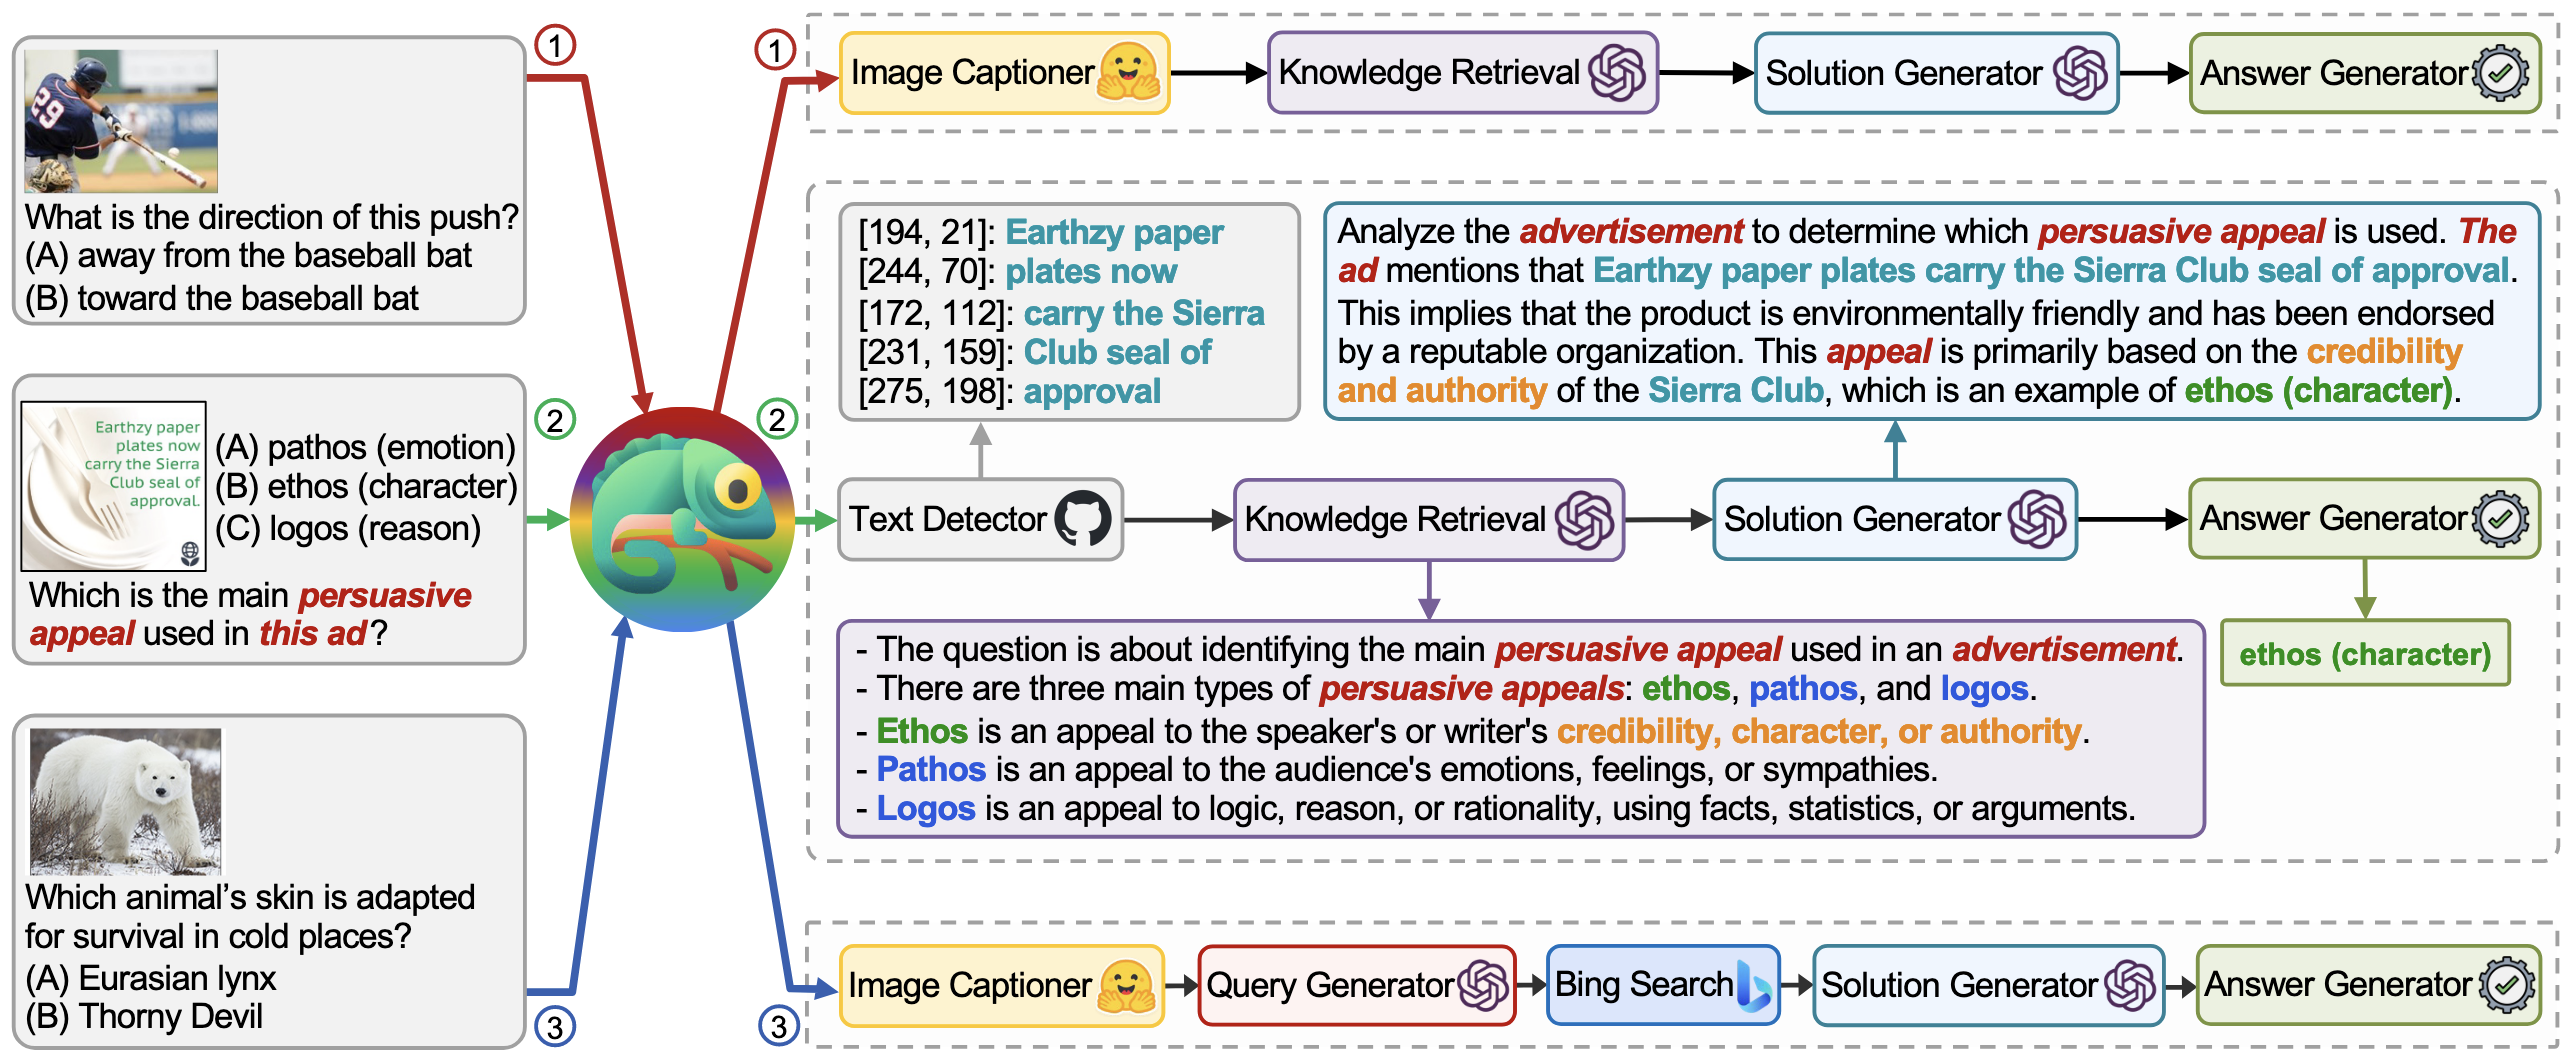
\includegraphics[width=1.0\textwidth]{figure/1.png}
\end{center}

{\fontsize{10}{14}\selectfont 
\begin{itemize}
    \item Goal: Dynamically selecting tools

    - GPT-4 works as planner with in-context learning \cite{gpt4}

    - Synthesize program with basic tools
\end{itemize}
}

\vspace{0.2cm}
\hrule
\printbibliography

\end{refsection}
\end{frame}
% ------------------ Slide 3 ------------------

\begin{frame}
\begin{refsection}

\begin{center}
    { \textbf{\textcolor{blue}{ {\fontsize{12}{14}\selectfont Related Work} }} }
\end{center}

\begin{itemize}
    \item LLM using tools

    - Codex was fine-tuned with Github codes \cite{codex}

    - Reasoning with coding was suggested \cite{PoT}

    \\[0.3cm]

    \item Limitation of prior works

    - Requires supervised fine-tuning

    - Fixed set of tools

    - Calls one tool at a time

    \\[0.3cm]

    \item Chameleon's difference

    - In-context learning without fine-tuning

    - Plug-and-play: adapt to new tools given description

    - Composes multi-step tool sequences

\end{itemize}

\vspace{0.2cm}
\hrule
\printbibliography

\end{refsection}
\end{frame}
% ------------------ Slide 4 ------------------

\begin{frame}

\begin{center}
    { \textbf{\textcolor{blue}{ {\fontsize{12}{14}\selectfont Comparision of work} }} }
\end{center}

\begin{center}
    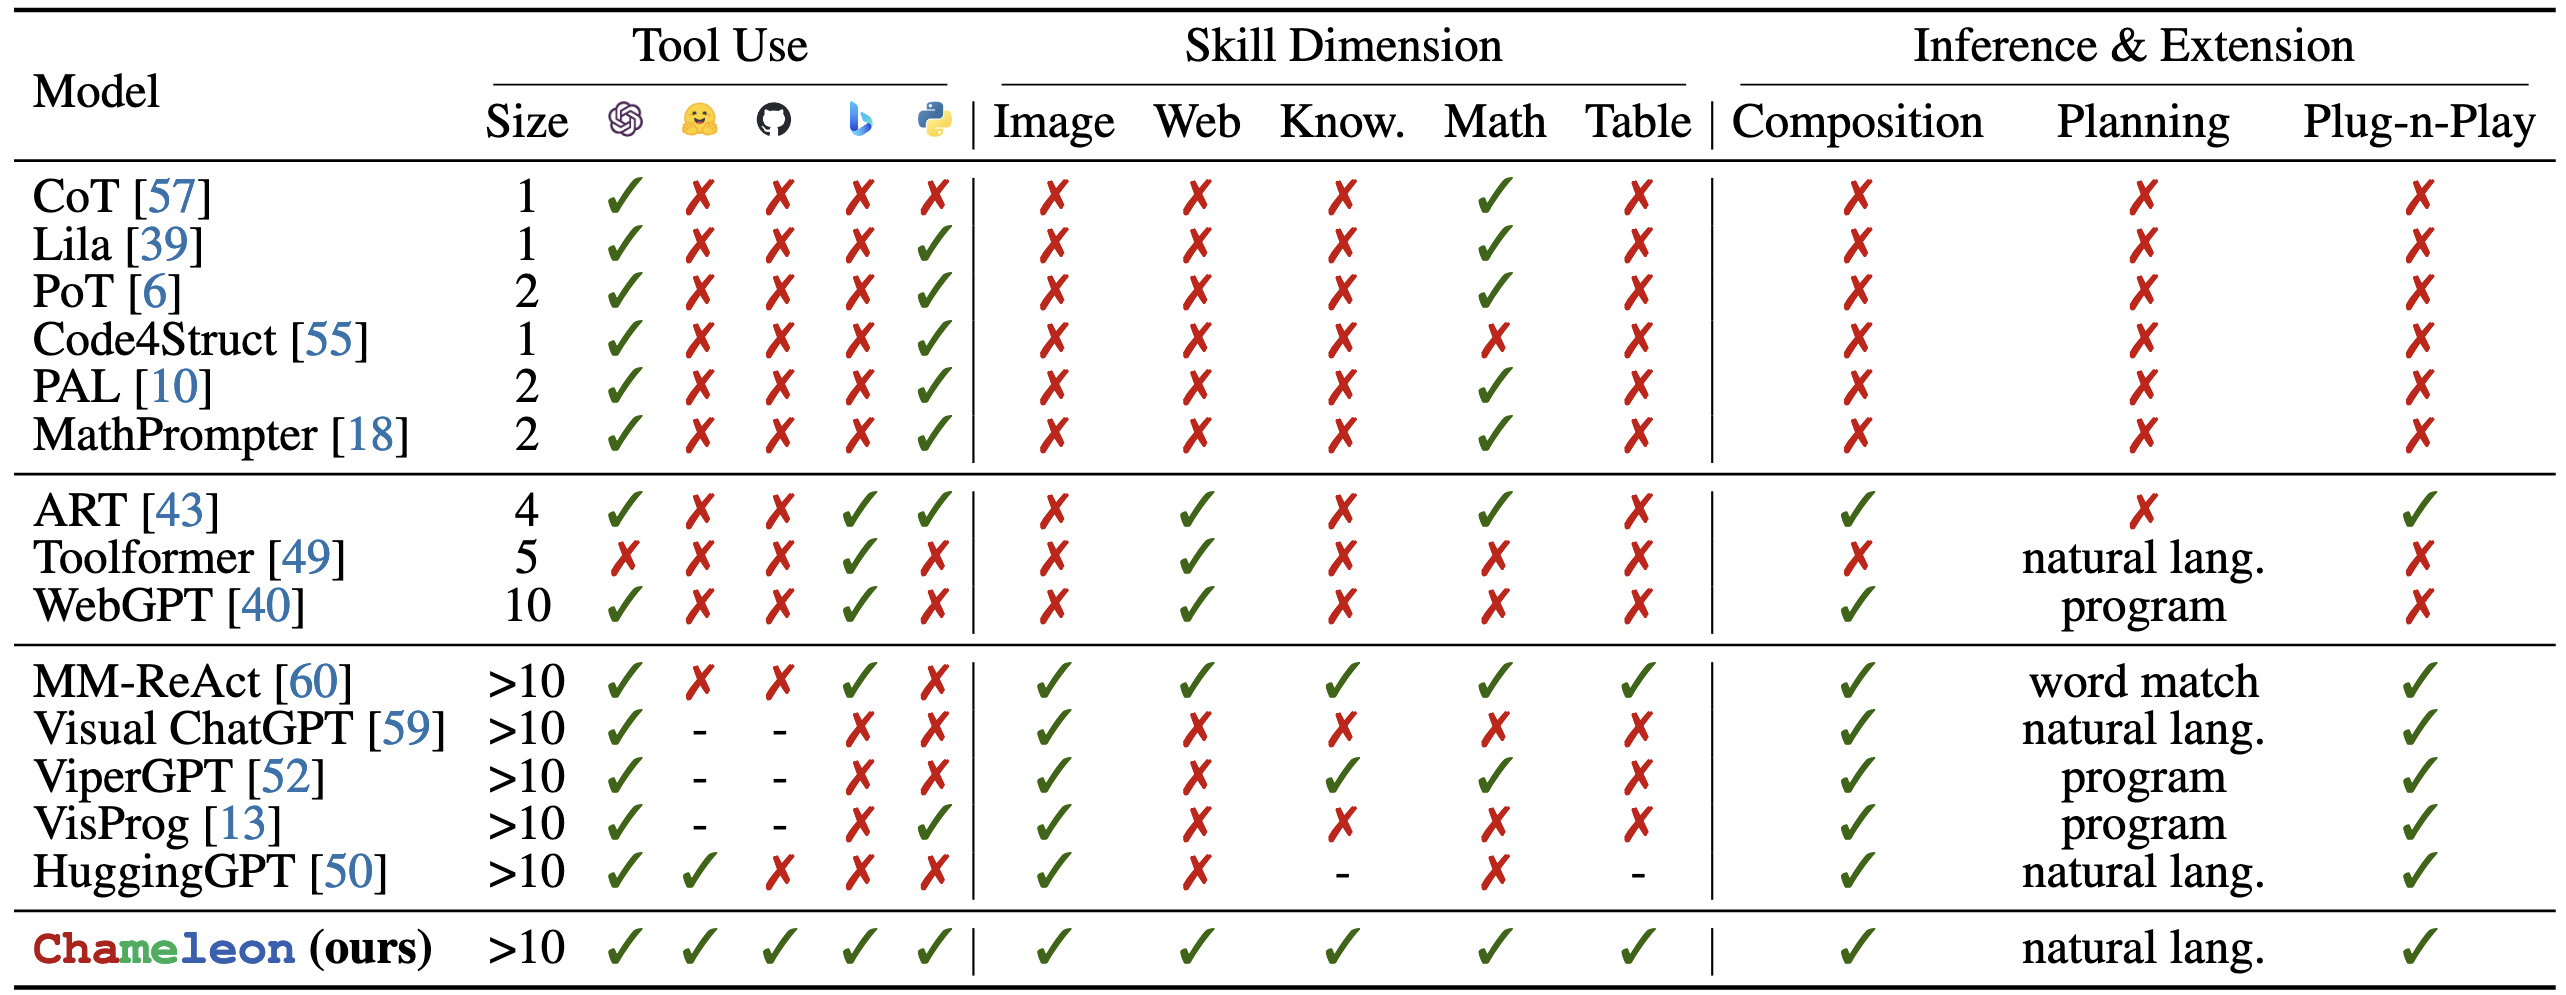
\includegraphics[width=1.0\textwidth]{table/1.png}
\end{center}

\begin{itemize}
    \item Prior Tools: Lack of generalization

    - Limited tools, Manually prompting usage

    \\[0.2cm]

    \item Our method: Chameleon

    - Plug-and-Play Flexibility

    - Natural language planning by LLM (Interpretable)

\end{itemize}

\end{frame}
% ------------------ Slide 5 ------------------

\begin{frame}

\begin{center}
    { \textbf{\textcolor{blue}{ {\fontsize{12}{14}\selectfont General Framework} }} }
\end{center}
\\[0.3cm]

\begin{itemize}
    \item Notations

    - Input query \( x_0 \)

    - Natural language planner \( \mathcal{P} \)

    - Task instruction \( \mathcal{I} \)

    - Module inventory \( \mathcal{M} \) consists of modules: \( \{ M_i \} \)

    - Constraints \( \mathcal{G} \) for the sequence orders of modules

    - Few-shot examples \( \mathcal{D} \)
\end{itemize}

\end{frame}
% ------------------ Slide 6 ------------------

\begin{frame}

\begin{center}
    { \textbf{\textcolor{blue}{ {\fontsize{12}{14}\selectfont General Framework} }} }
\end{center}
\\[0.3cm]

\begin{itemize}
    \item Workflow

    - Plan \(p\), Time step \(t\), Output \(y^t\), Cache \(c^t\)

    - \( p = \mathcal{P}(x_0; \mathcal{I}, \mathcal{M}, \mathcal{G}, \mathcal{D}) \)

    - \(y^t \leftarrow M^t(x^{t-1};c^{t-1})\)

    - \(x^t \leftarrow \) update\_input\( (x^{t-1};y^t) \)

    - \(c^t \leftarrow \) update\_cache\( (c^{t-1};y^t) \)

    - The functions are hand-designed for each \(M_i\)

    \\[0.5cm]   

    \item Response

    - \( r=y^T \leftarrow M^T(x^{T-1};c^{T-1}) \)
\end{itemize}

\end{frame}
% ------------------ Slide 7 ------------------

\begin{frame}

\begin{center}
    { \textbf{\textcolor{blue}{ {\fontsize{12}{14}\selectfont Module Inventory} }} }
\end{center}

\begin{center}
    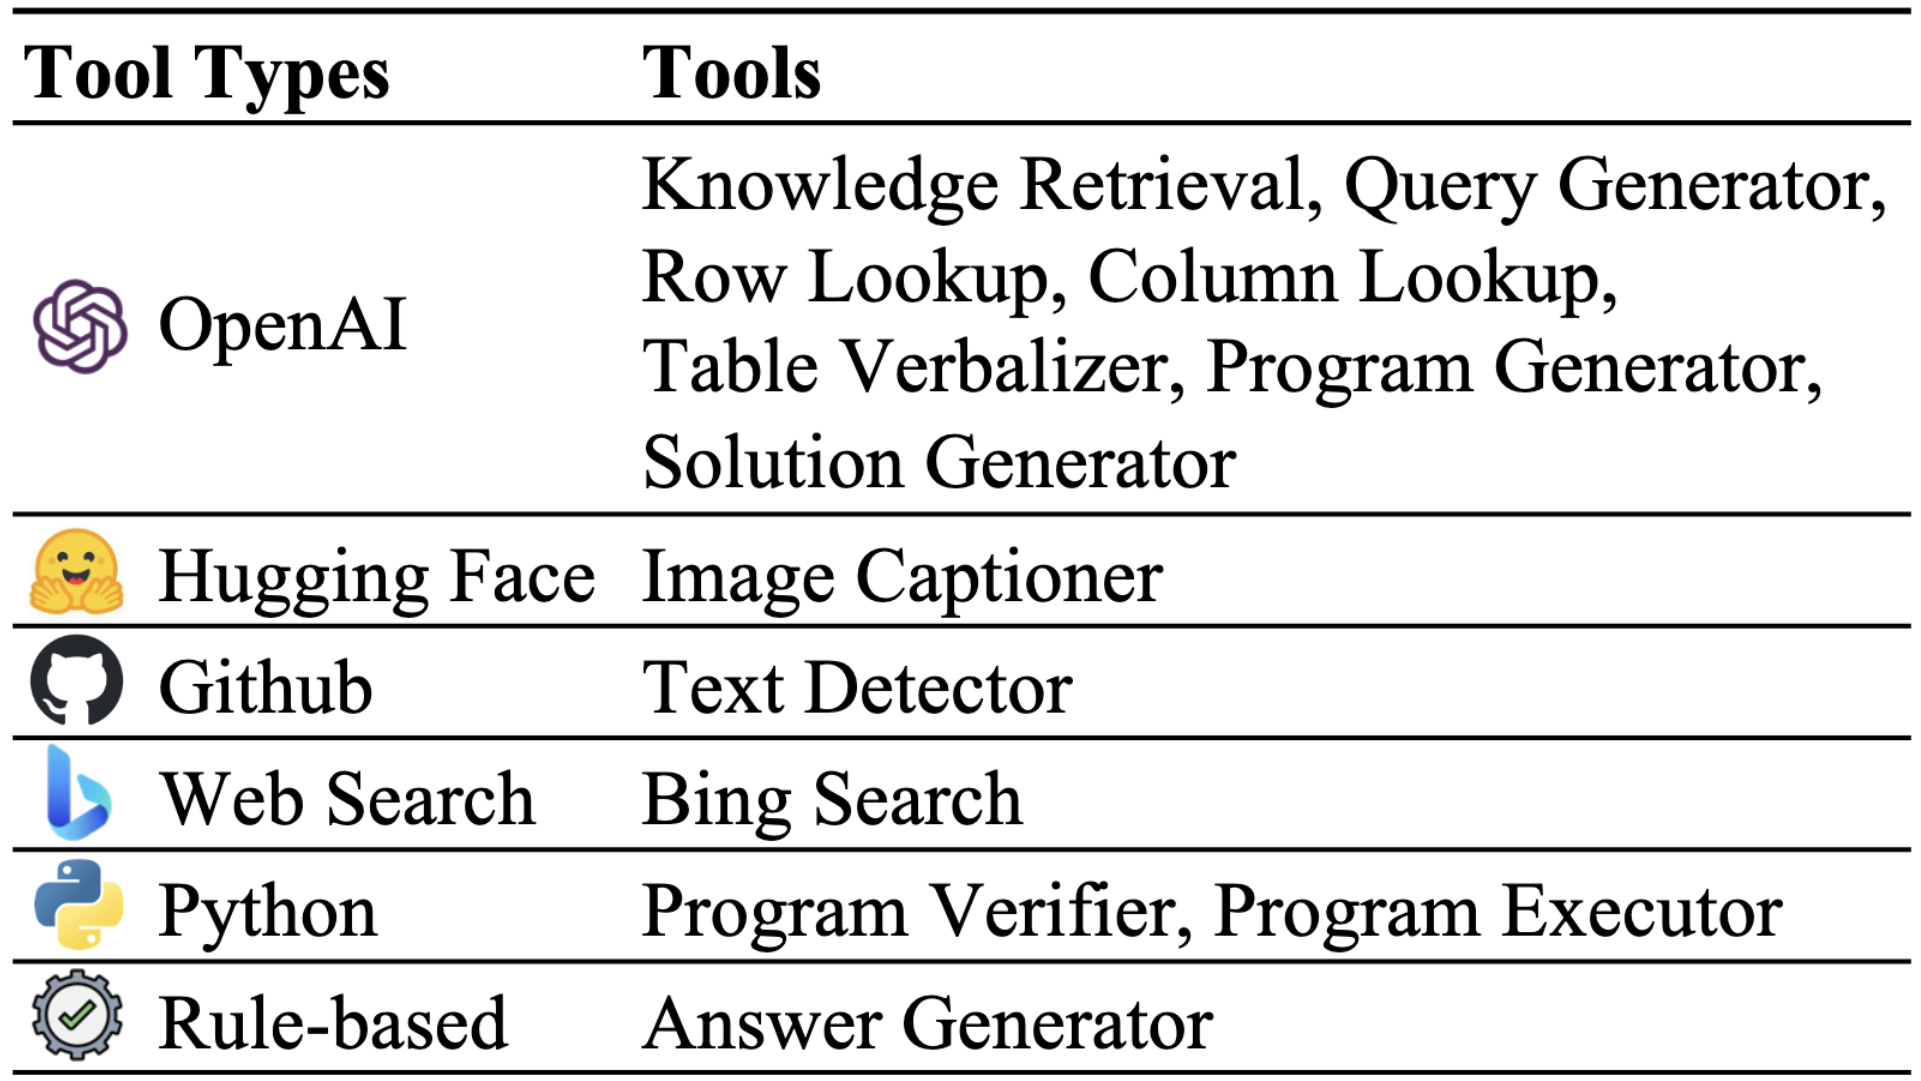
\includegraphics[width=0.6\textwidth]{table/2.png}
\end{center}

\begin{itemize}
    \item Knowledge Retrieval

    - This module retrieves additional background knowledge

    \item Query Generator

    - It creates search engine queries based on the problem

    \item Row / Column Lookup

    - Reasoning process may involve tabular context

    - Focusing only on relevant section for query
\end{itemize}

\end{frame}
% ------------------ Slide 8 ------------------

\begin{frame}

\begin{center}
    { \textbf{\textcolor{blue}{ {\fontsize{12}{14}\selectfont Module Inventory} }} }
\end{center}

\begin{center}
    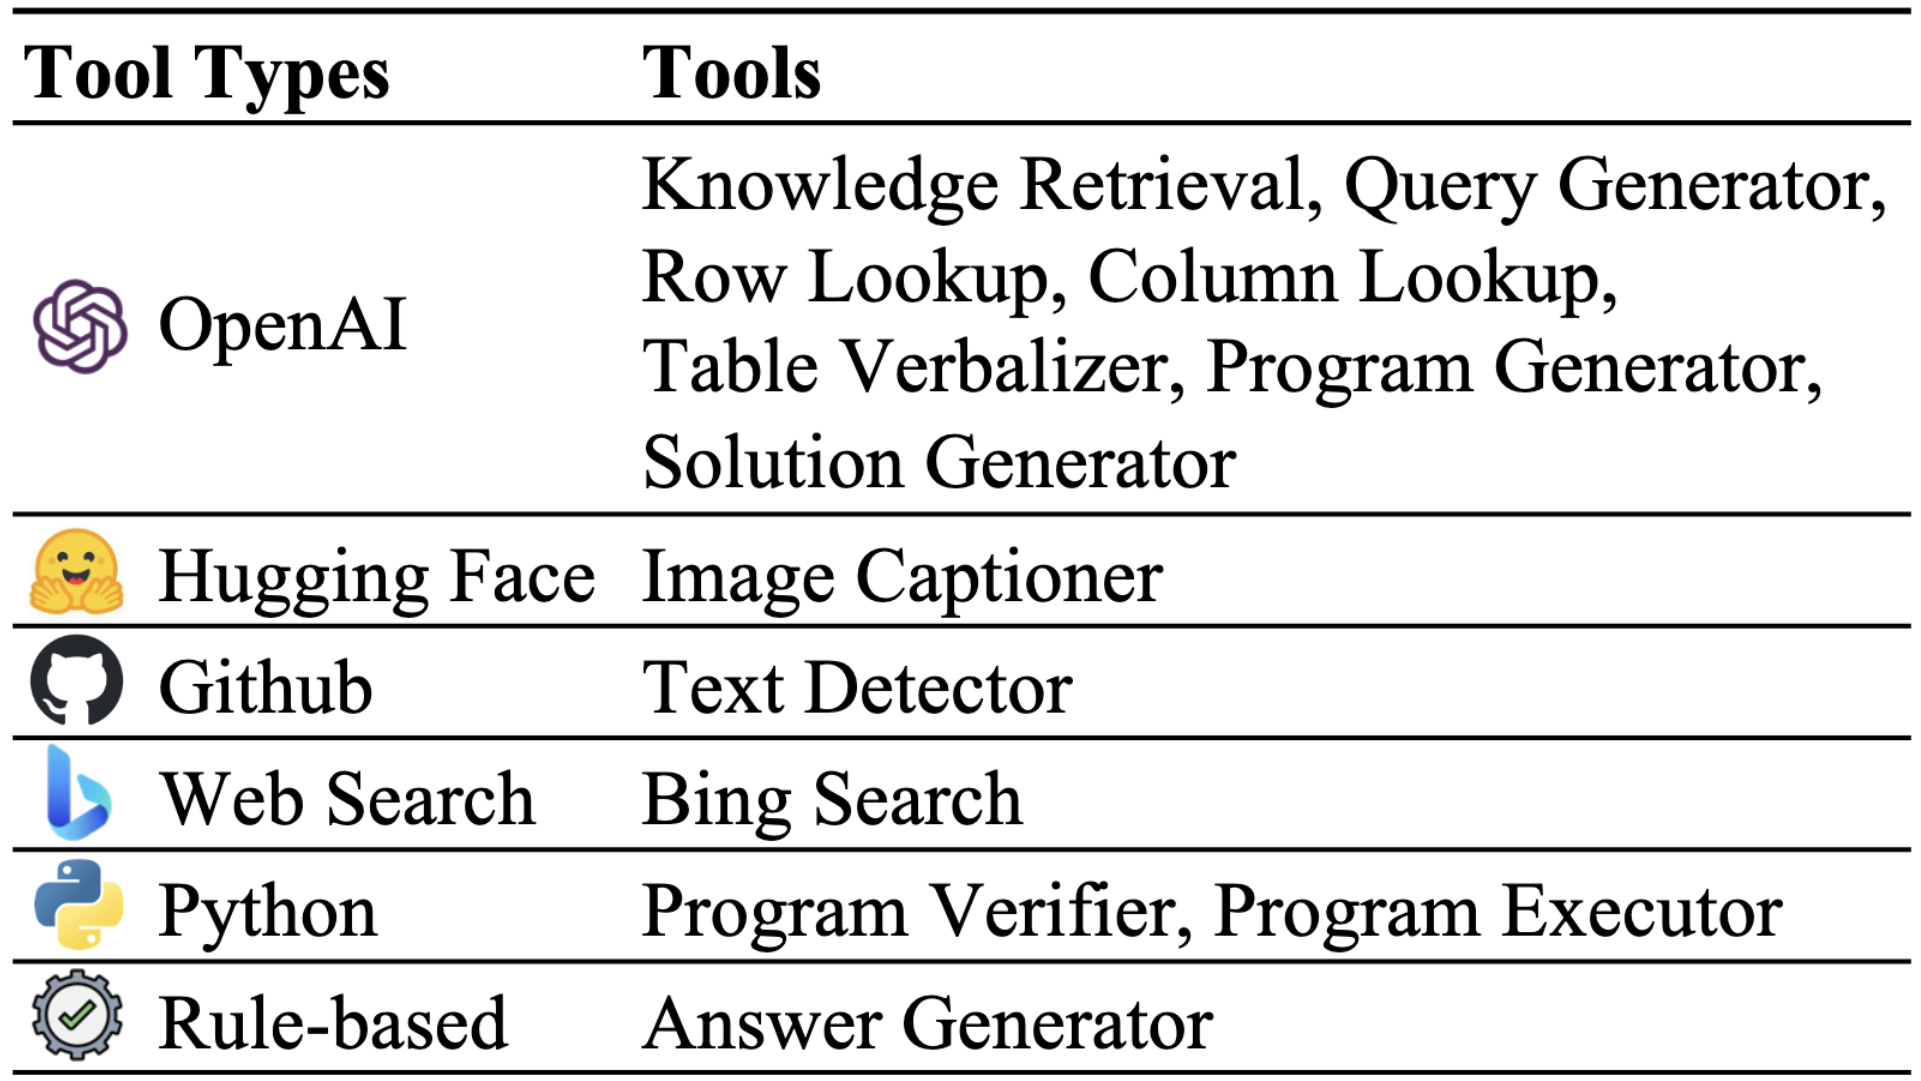
\includegraphics[width=0.6\textwidth]{table/2.png}
\end{center}

\begin{itemize}
    \item Table Verbalizer

    - Converting structured tables into text

    \\[0.3cm]

    \item Program Generator

    - It generates Python programs to solve queries
\end{itemize}

\end{frame}
% ------------------ Slide 9 ------------------

\begin{frame}

\begin{center}
    { \textbf{\textcolor{blue}{ {\fontsize{12}{14}\selectfont Module Inventory} }} }
\end{center}

\begin{center}
    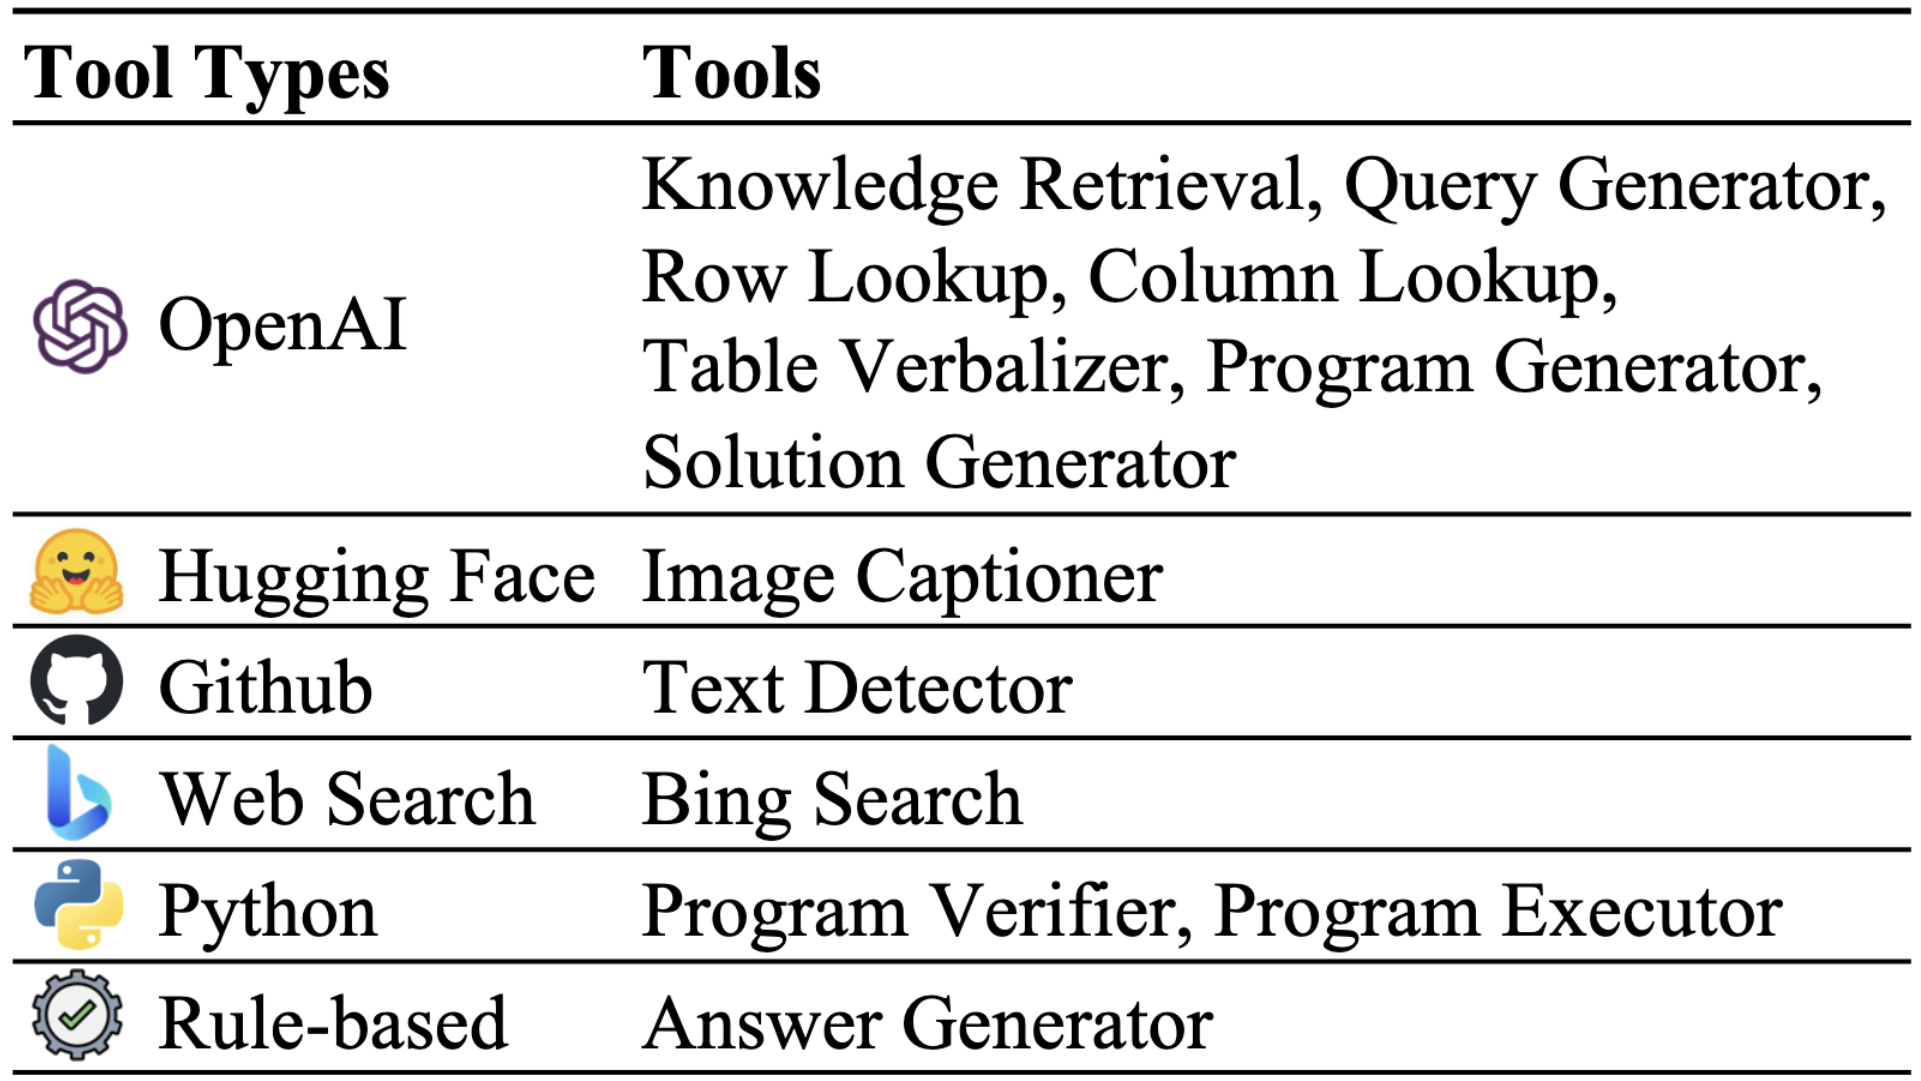
\includegraphics[width=0.6\textwidth]{table/2.png}
\end{center}

\begin{itemize}
    \item Image Captioner

    - Converts raw image data into a textual description

    \item Text Detector

    - Identifies text within a given image

    \item Bing search

    - It excels when broader or up-to-date information
\end{itemize}

\end{frame}
% ------------------ Slide 10 ------------------

\begin{frame}
\begin{refsection}

\begin{center}
    { \textbf{\textcolor{blue}{ {\fontsize{12}{14}\selectfont Module Inventory} }} }
\end{center}

\begin{center}
    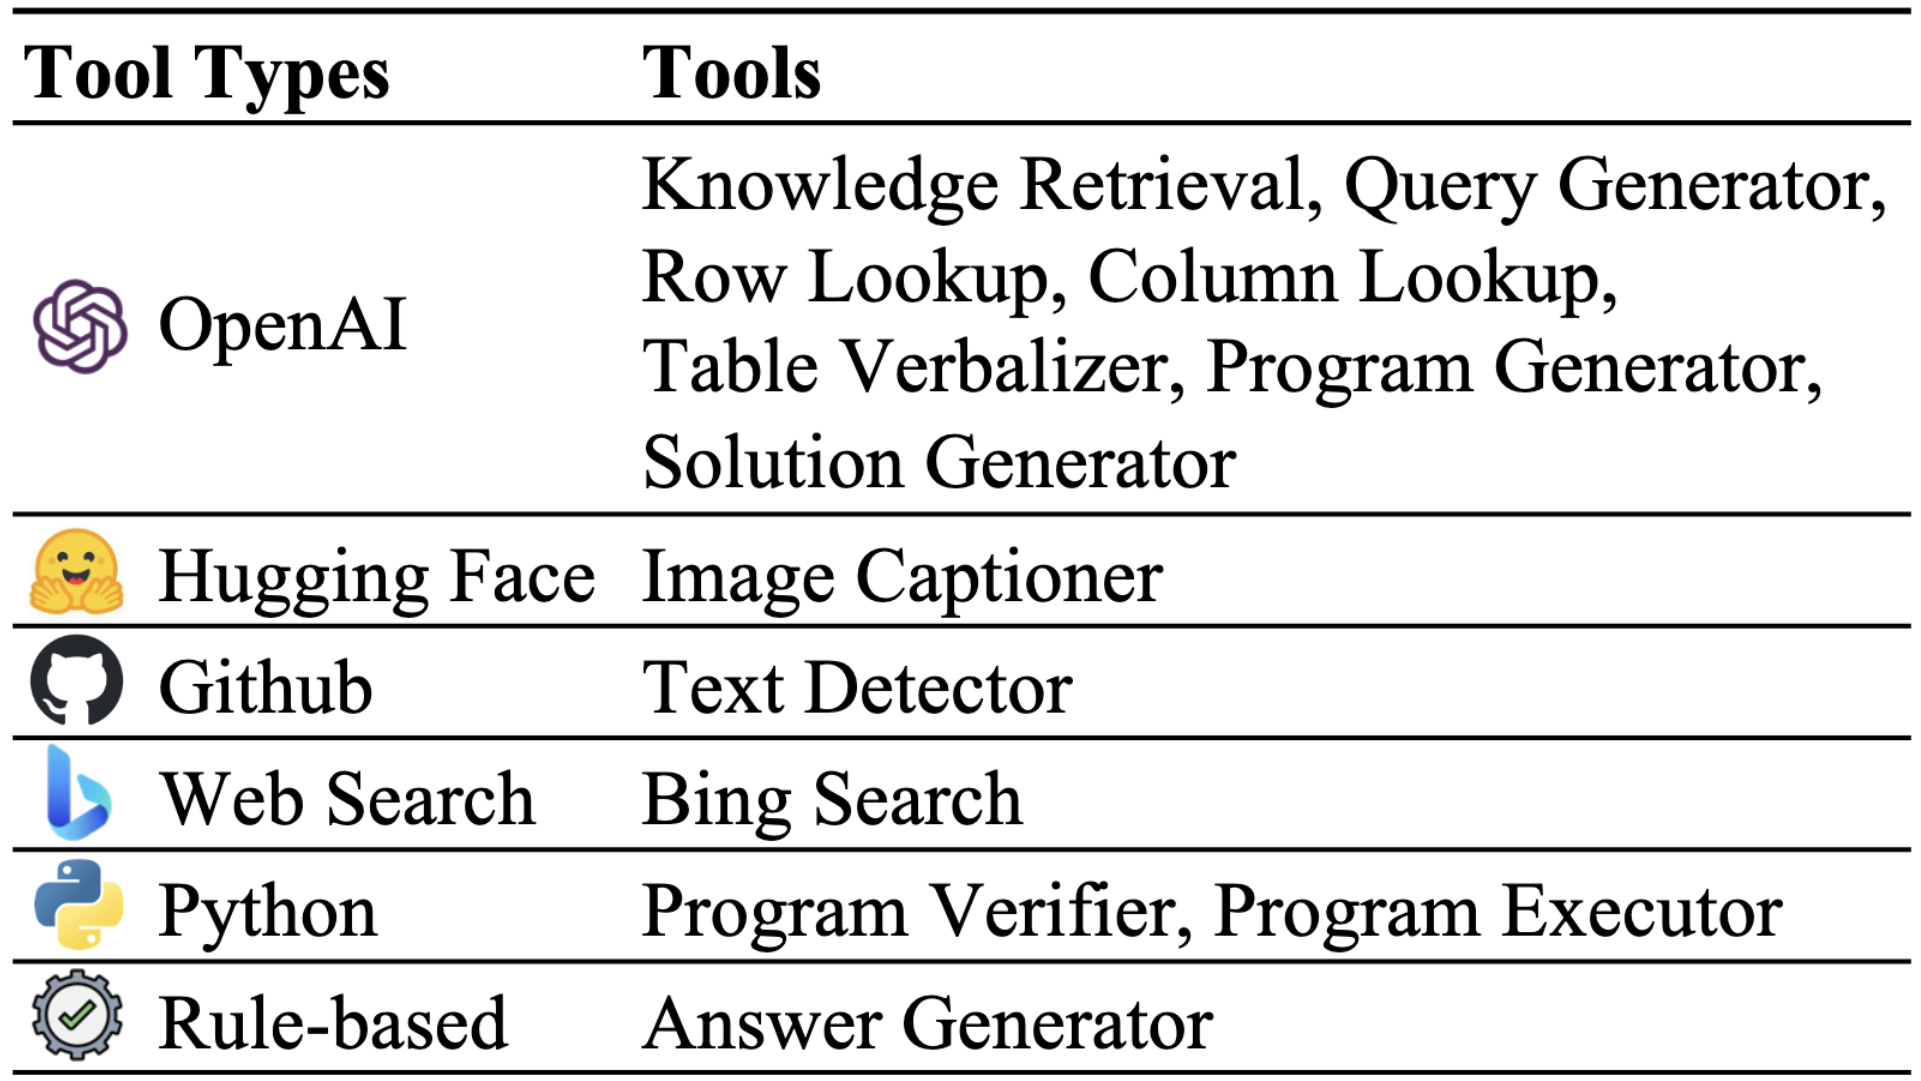
\includegraphics[width=0.6\textwidth]{table/2.png}
\end{center}

\begin{itemize}
    \item Program Verifier

    - Checks for syntax and logical errors \cite{self-refine}

    \item Program Executor

    - Executes the program and produces the result
\end{itemize}

\vspace{0.3cm}
\hrule
\printbibliography

\end{refsection}
\end{frame}
% ------------------ Slide 11 ------------------

\begin{frame}
\begin{refsection}

\begin{center}
    { \textbf{\textcolor{blue}{ {\fontsize{12}{14}\selectfont Module Inventory} }} }
\end{center}

\begin{center}
    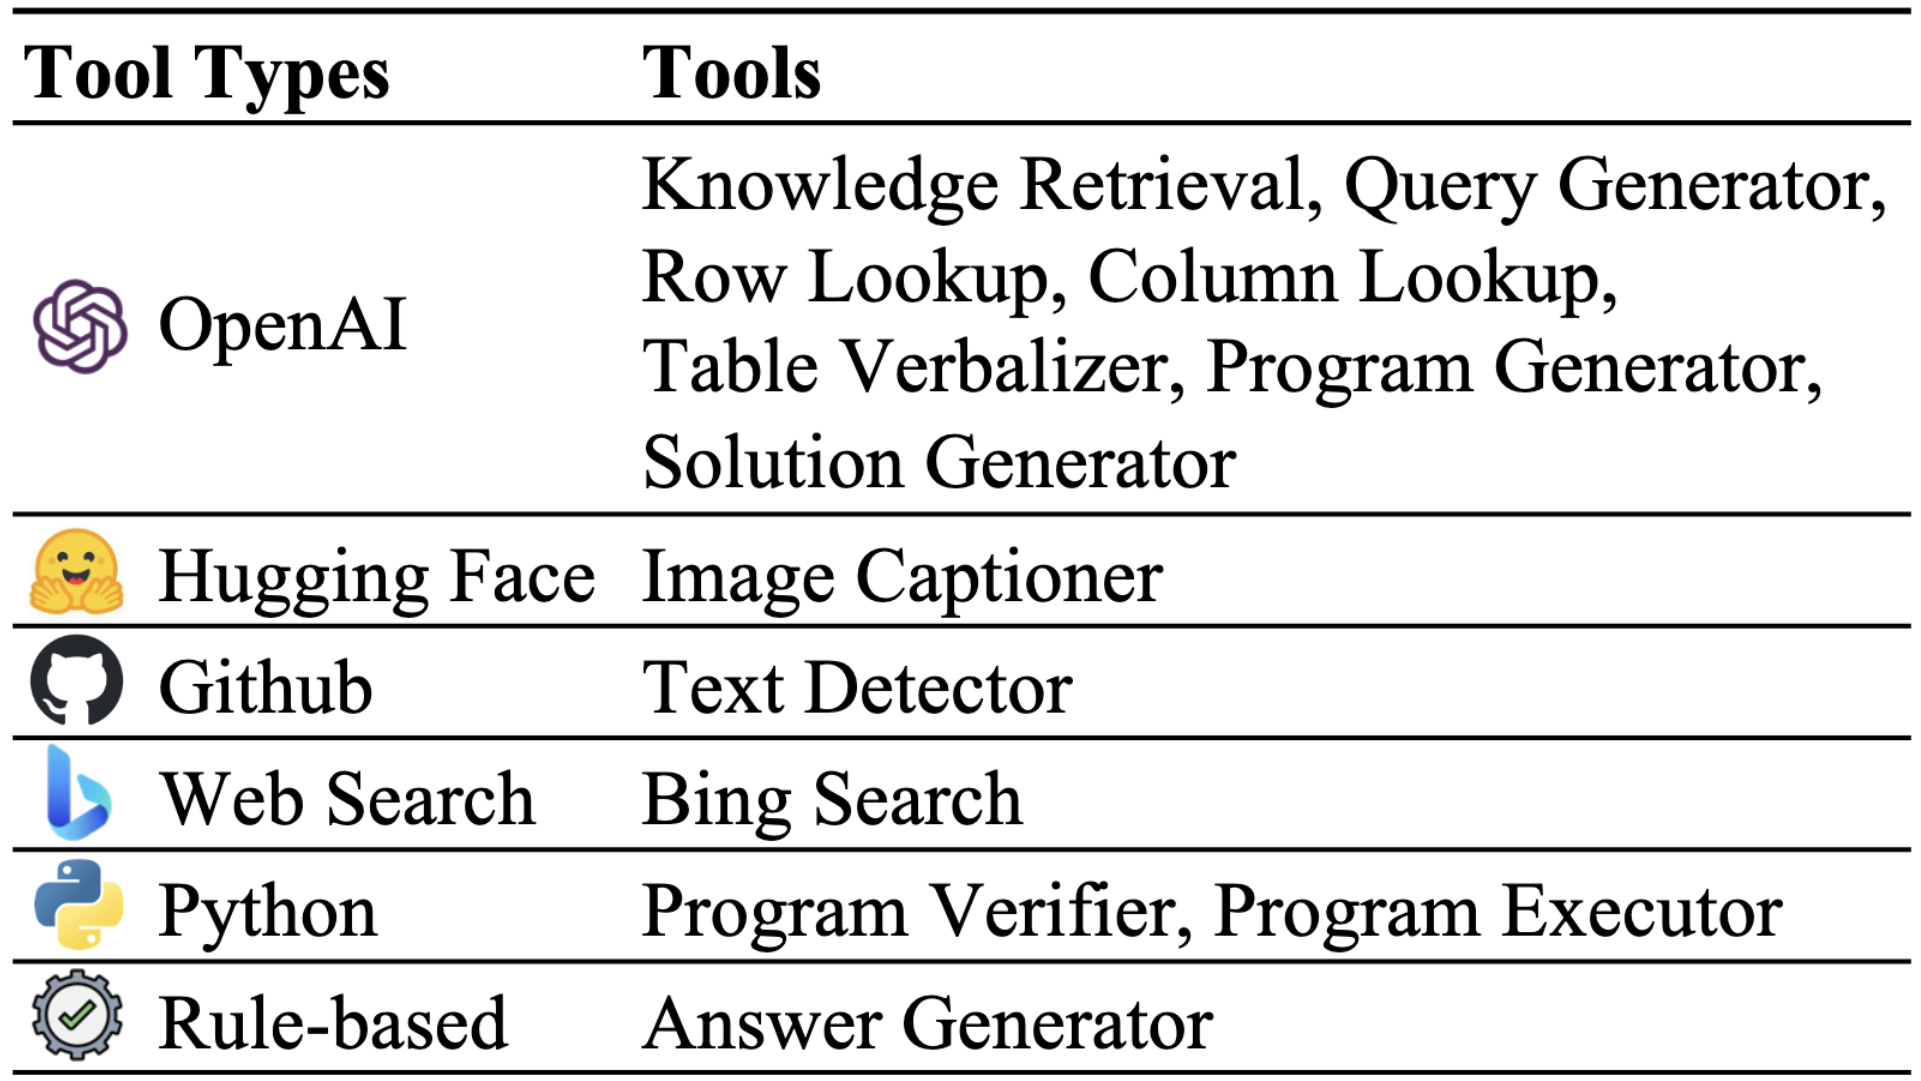
\includegraphics[width=0.6\textwidth]{table/2.png}
\end{center}

\begin{itemize}
    \item Solution Generator

    - Using all the cached information, generate solution \cite{CoT}

    \item Answer Generator

    - Executes the program and produces the result
\end{itemize}

\vspace{0.3cm}
\hrule
\printbibliography

\end{refsection}
\end{frame}
% ------------------ Slide 12 ------------------

\begin{frame}
\begin{refsection}

\begin{center}
    { \textbf{\textcolor{blue}{ {\fontsize{12}{14}\selectfont Benchmark} }} }
\end{center}
\\[0.5cm]

{\fontsize{10}{14}\selectfont 
\begin{itemize}
    \item TabMWP \cite{TabMWP}

    - A math reasoning benchmark with tables

    - Row \& Column lookup, Table Verbalizer would be needed

    \\[0.5cm]
    
    \item ScienceQA \cite{ScienceQA}

    - A multi-modal dataset covering scientific topics

    - e.g.) Physics problem with image

\end{itemize}
}

\vspace{0.5cm}
\hrule
\printbibliography

\end{refsection}
\end{frame}
% ------------------ Slide 13 ------------------

\begin{frame}

\begin{center}
    { \textbf{\textcolor{blue}{ {\fontsize{12}{14}\selectfont Experiment} }} }
\end{center}
\\[0.3cm]

\begin{center}
    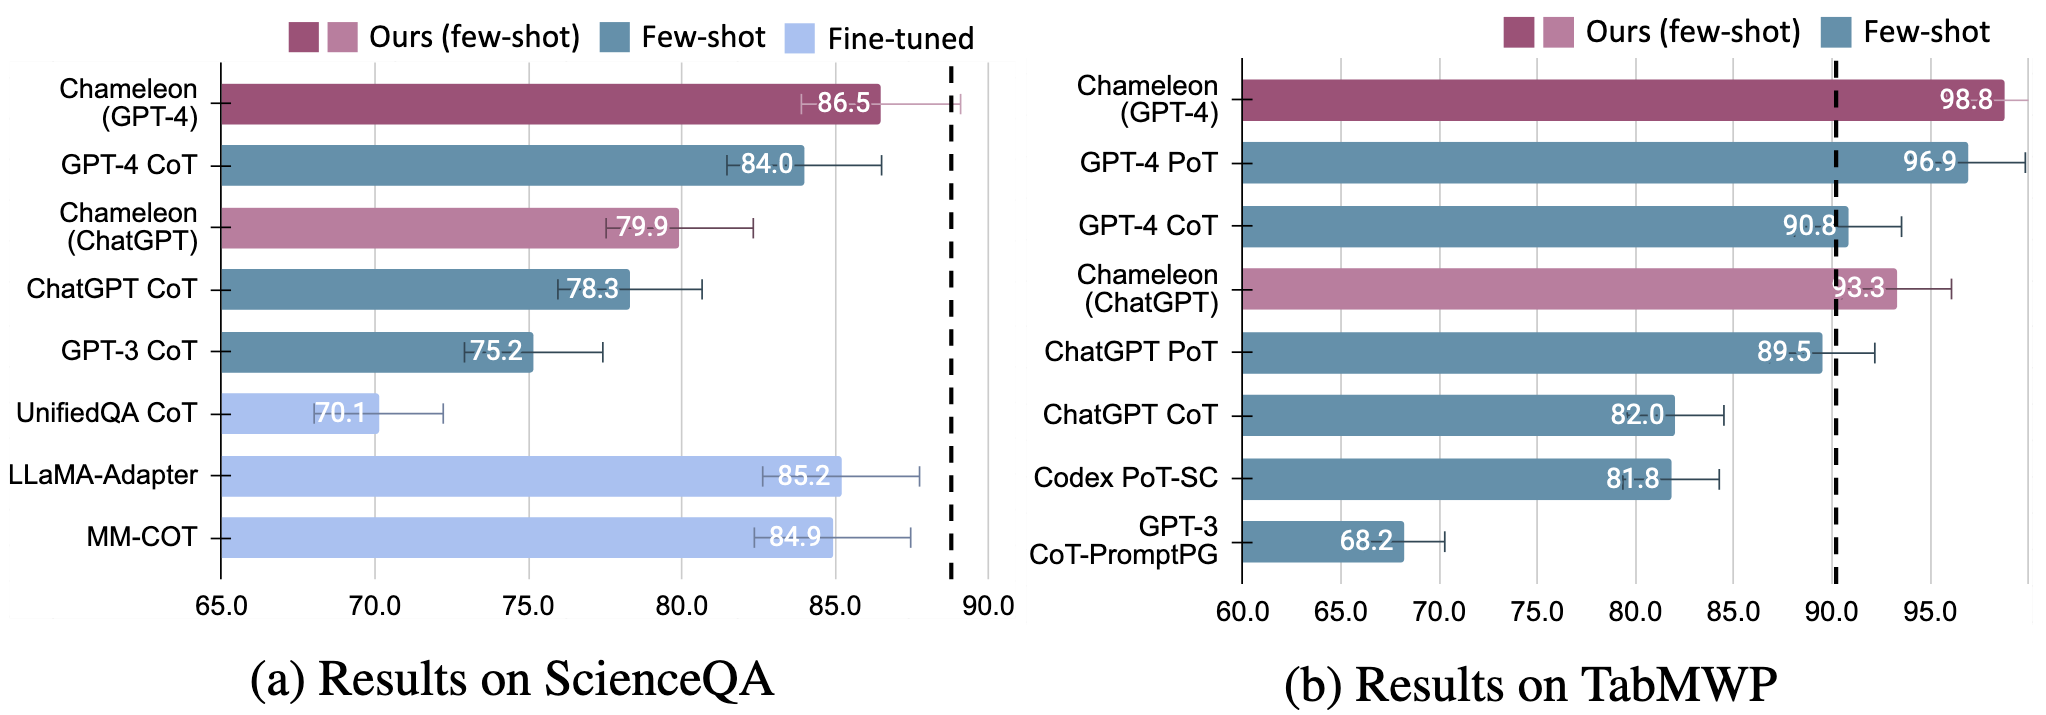
\includegraphics[width=1.0\textwidth]{figure/3.png}
\end{center}


{\fontsize{10}{14}\selectfont 
\begin{itemize}
    \item Result
    
    - SOTA in few-shot settings (ScienceQA)

    - Outperformed fine-tuning models (TabMWP)
\end{itemize}
}

\end{frame}
% ------------------ Slide 14 ------------------

\begin{frame}

\begin{center}
    { \textbf{\textcolor{blue}{ {\fontsize{12}{14}\selectfont Experiment} }} }
\end{center}
\\[0.3cm]

\begin{center}
    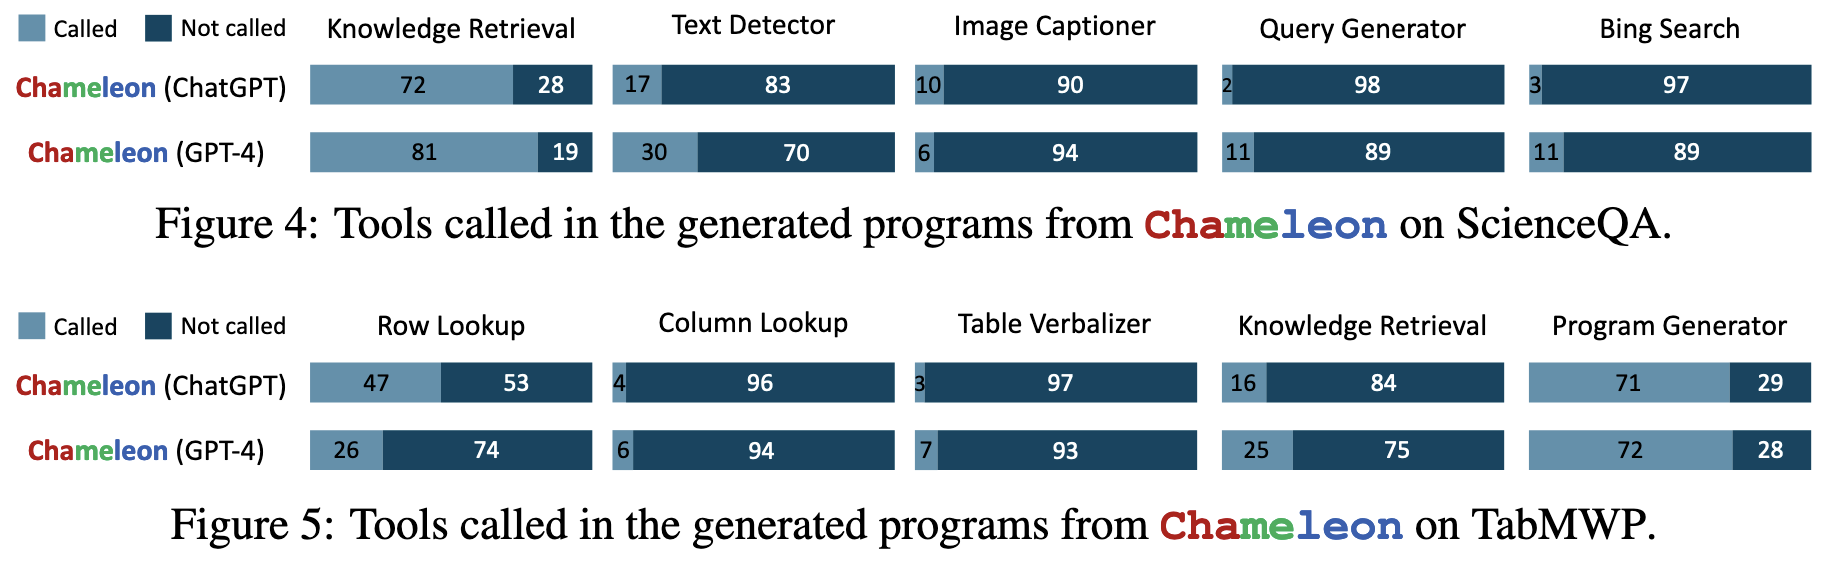
\includegraphics[width=1.0\textwidth]{figure/4-5.png}
\end{center}


{\fontsize{10}{14}\selectfont 
\begin{itemize}
    \item Tool usage of ChatGPT-based Chameleon
    
    - Heavily influenced by few-shot examples

    - Strongly prefers certain tools

    \\[0.3cm]

    \item Tool usage of GPT-4-based Chameleon

    - Distributes tool calls more objectively

    - Uses query generator and web search at the same time
\end{itemize}
}

\end{frame}
% ------------------ Slide 15 ------------------

\begin{frame}

\begin{center}
    { \textbf{\textcolor{blue}{ {\fontsize{12}{14}\selectfont Ablation study} }} }
\end{center}
\\[0.3cm]

\begin{center}
    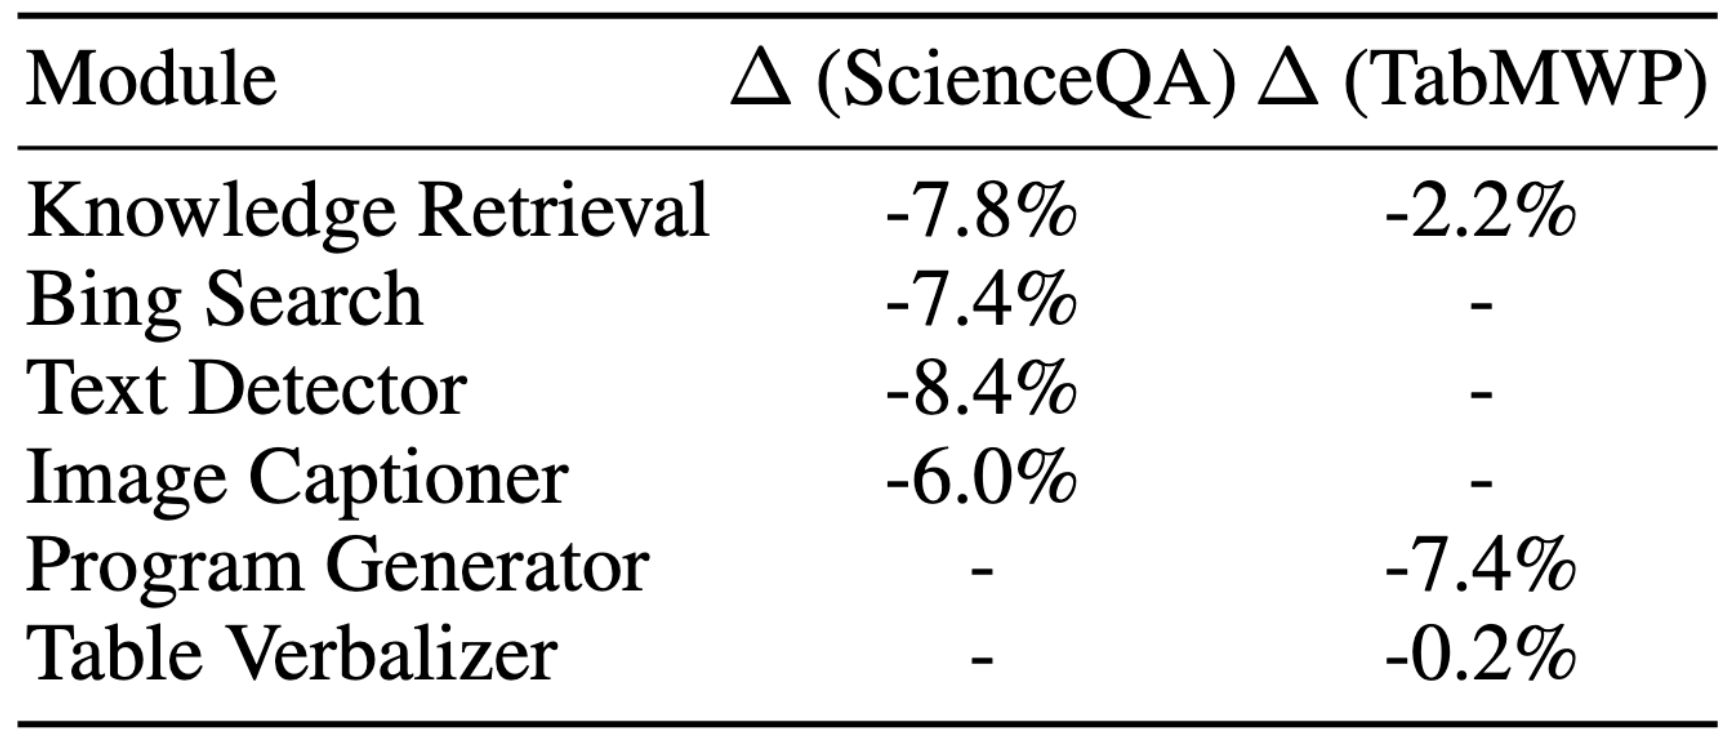
\includegraphics[width=0.8\textwidth]{table/5.png}
\end{center}


{\fontsize{10}{14}\selectfont 
\begin{itemize}
    \item Most of tools are vital
    
    - Knowledge retrieval is important in both tasks

    - Domain specific tools are important

    - Vision models for ScienceQA, Program tools for TabMWP
\end{itemize}
}

\end{frame}
% ------------------ Slide 15 ------------------

\begin{frame}

\begin{center}
    { \textbf{\textcolor{blue}{ {\fontsize{12}{14}\selectfont Error Analysis} }} }
\end{center}
\\[0.3cm]

\begin{center}
    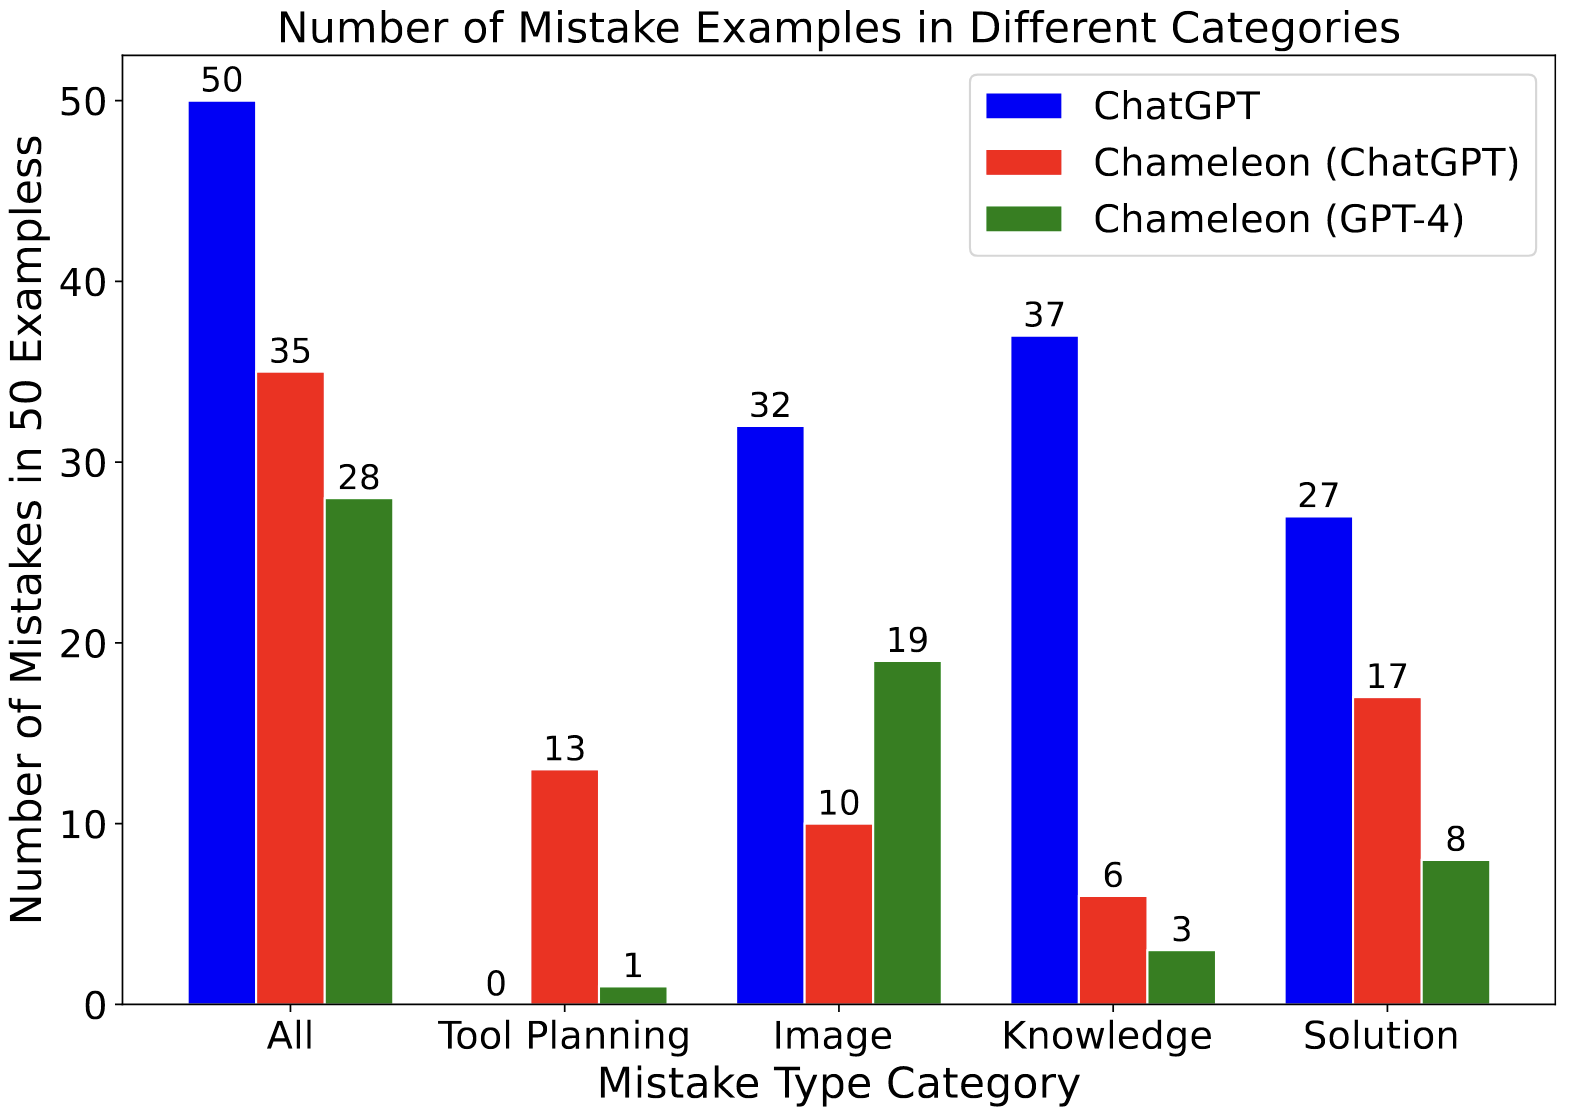
\includegraphics[width=0.7\textwidth]{figure/6.png}
\end{center}


{\fontsize{10}{14}\selectfont 
\begin{itemize}
    \item 50 mistakes of ChatGPT on ScienceQA
    
    - Chameleon reduces mistakes by tools
\end{itemize}
}

\end{frame}
% ------------------ Slide 16 ------------------

\begin{frame}

\begin{center}
    { \textbf{\textcolor{blue}{ {\fontsize{12}{14}\selectfont Conclusion} }} }
\end{center}
\\[0.3cm]

{\fontsize{10}{14}\selectfont 
\begin{itemize}
    \item We introduce \textit{Chameleon}

    - Augmenting external tools

    - Plug-and-play manner

    \\[0.5cm]

    \item Experiments on ScienceQA, TabMWP

    - Significant improvements in accuracy

    - Potential for addressing real-world queries
\end{itemize}
}

\end{frame}
% ------------------ Slide 17 ------------------
\end{document}
